% Chapter 1

\chapter{Segmentation of the Inferior Alveolar Canal: an overview}

\lhead{Chapter 1. \emph{Segmentation of the Inferior Alveolar Canal}} % This is for the header on each page - perhaps a shortened title
\label{chp:overview}
%----------------------------------------------------------------------------------------

\def\:{\hskip0pt} %Definisce un modo veloce per permettere a latex di sillabare correttamente anche parole come 4-connectivity. Il corretto utilizzo è il seguente: 4\:-\:connectivity.

\section{Introduction}
Dental implant placement within the jawbone is a routine surgical procedure that
can become complicated due to the presence of the Inferior Alveolar Nerve (IAN)
nearby. The nerve, in particular, is frequently in close proximity to the roots
of molars, and its position must thus be meticulously detailed prior to surgical
removal. Avoiding contact with the IAN is a primary concern during these
operations, thus its segmentation is crucial in surgical planning. Today the
standard de-facto is to take a CBCT scan of the jawbone and a 2D panoramic view
is extracted. This view allows medical experts to depict the IANs position with
line. We refer to this type of annotation as \emph{sparse} or \emph{2D}
annotation. A 3D annotation of the IAC is often avoided as it would require a
huge amount of time, but this type of segmentation would offer a much more
precise knowledge of the position of the IAN and IAC and could allow dentists to
plan a more detailed surgical approach. For this reason, a lot of research about
automatic segmentation of the IAC has been carried out and is still active
today.\\

In this chapter, we first describe in detail the role of the IAN and the IAC,
what a CBCT is and the definitions and characteristics of different types of
segmentations, to give a brief introduction on which are the main components of
the final work. In the following chapter, we will look at the main components
used to perform image segmentation in the medical field, until today state of
the art. Next in chapter 3, we will detail the dataset that has been used, by
describing how it has been created, preprocessed, and some other thoughts. In
chapter 4, the network I've used as starting point and the benefits obtained by
refactoring the code. Finally, in chapter 5, we will discuss the different
approaches taken to try to improve the current state of the art, the results
obtained and some of the possible future works.

\section{Inferior Alveolar Canal}
The Inferior Alveolar Canal (IAC) is a small passageway shaped as a tube that
runs through the lower jawbone. It houses the Inferior Alveolar Nerve (IAN),
which is responsible for transmitting sensory information from the teeth, gums,
and lips to the brain. It also provides motor innervation to the muscles of
mastication (i.e. the muscles responsible for chewing). Dentists need to be able
to accurately locate the IAC before performing certain surgical operations, such
as tooth extractions or placement of dental implants. This is because the IAC is
located very close to the roots of the teeth, and damage to the IAC during
surgery can result in permanent nerve damage which would cause numbness,
tingling, and pain in the affected area. In severe cases, it can also lead to
muscle weakness and paralysis.

\section{Cone Beam Computed Tomography}
Cone beam computed tomography (CBCT) is a medical imaging technique consisting
of X-ray computed tomography where rays are divergent, forming a cone. This type
of computed tomography is well suited for imaging the craniofacial area as it
provides clear images of highly contrasted structures, very helpful to evaluate
bones. It has become common in dentistry such as oral surgery, endodontics, and
orthodontics.
The main reasons and advantages of CBCT concerning other CTs are:
\begin{enumerate}
  \item{\textbf{X-ray beam limitation:} reducing the size of the irradiated area
  by collimating the primary x-ray beam to the area of interest minimizes the
  radiation dose. Most CBCT units can be adjusted to scan small regions for
  a specific diagnostic task. They are also able to scan the whole craniofacial
  structure if needed.}
  \item{\textbf{Image accuracy:} We created a novel, large, and publicly
  available maxillo-facial CBCT (Cone Beam Computed Tomography) dataset, with 2D
  and 3D manual annotations, provided by expert clinicians. All CBCT units
  provide voxel resolutions that are isotropic (i.e. equals in all the 3
  dimensions) while in conventional CT, voxels are anisotropic (i.e. rectangular
  cubes).}
  \item{\textbf{Rapid scan time:} CBCT acquires all the basis images in a single
  rotation, thus scan time goes from 10s to 70s. Although faster scanning time
  usually means fewer basis images from which to reconstruct the volumetric
  dataset, motion artifacts due to subject movement are reduced.}
\end{enumerate}
These advantages come with some drawbacks: Hounsfield units (HU) is the metric
used to determine the radiodensity of tissue analyzed. In the Hounsfield scale,
numbers go from values of $-1000$ for air to values of $1600$ for dense bones.
In CBCT scans, the radiodensity is inaccurate because different areas in the
scan appear with different greyscale values depending on their relative
positions in the organ being scanned, despite possessing identical densities,
because the image value of a voxel of an organ depends on the position in the
image volume. HU measured from the same anatomical area with both CBCT and
medical-grade CT scanners are not identical and are thus unreliable for
determination of site-specific, radiographically-identified bone density for
purposes such as the placement of dental implants, as there is "no good data to
relate the CBCT HU values to bone quality" \cite{Miles2007}.\\
The images resulting from CBCT scans are usually exported as DICOM (Digital
Imaging and Communications in Medicine) which is the standard used worldwide to
store, exchange, and transmit medical images.

\section{DICOM file format}
TODO?

\section{Image Segmentation}
Image segmentation is a well-known topic in computer and image processing with a
wide range of applications, such as medical imaging, robotics, video
surveillance, etc.
It involves partitioning images into one or more objects and can also include
classifying these objects. Many traditional algorithms have been developed in
the literature but, in the most recent years, they have all been dominated by
deep neural networks. Since 2015 a huge amount of different types of networks
that aim to perform image segmentation have been proposed for each field where
it's needed.
Before presenting how nowadays segmentation is performed, we must state which
are the different types of segmentation that have been classified:

\begin{itemize}
  \item{\textbf{Semantic segmentation:} Semantic Segmentation performs a
    pixel-by-pixel classification with a predefined set of object categories for
    all the pixels of the images. In practice, given a RGB image
    (\texttt{height} $\times$ \texttt{width} $\times$ \texttt{3}) we output a
    segmentation map of size (\texttt{height} $\times$ \texttt{width} $\times$
    \texttt{classes}) where each value corresponds to which class the same pixel
    in the original images belong.}

  \item{\textbf{Instance segmentation:} One possible issue of semantic
    segmentation is that it doesn't allow distinguishing two or more objects of
    the same class when they overlap in the image. Instance segmentation
    overcomes this problem by outputting a different number of channels based on
    the number of instances present in the image.}

  \item{\textbf{Panoptic segmentation:} The latter type of segmentation is
    called Panoptic segmentation and is the result of the previously presented
    method joined together. The difference with the instance segmentation is
    that in this case instances are not allowed to overlap then for a single
    pixel, a single instance must be assigned.}
\end{itemize}

% Figure 1: example of segmentation on mri image
\begin{figure}[h]
  \centering
  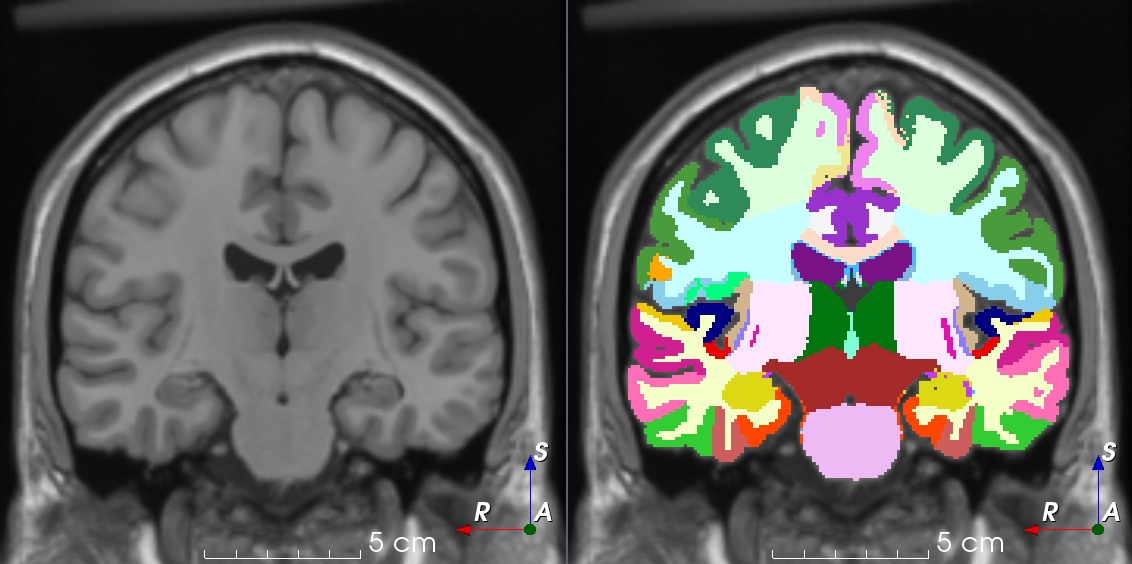
\includegraphics[width=0.8\textwidth]{Images/example_segmentation.png}
  \caption{Example of a multiclass semantic segmentation, different colors
  represent different classes}
  \label{fig:segmentation}
\end{figure}



% \section{Segmentation using Deep Neural Networks}
% As stated before, nowadays deep learning is the dominant method used for
% segmentation. Convolutional Neural Networks are still the most used type of
% networks used to date but new promising techniques, such as Graph Neural Networks or
% Transformers, are always more and more used.

